We leveraged the confirmed cases in the COVID-19 Open Research dataset~\cite{covid19weather} to calculate the daily growth rate and average growth rate. The number of confirmed cases in each region is treated as a random variable, and the recorded value in the dataset is a set of random samples.
For each region in China, we used~\cref{eq:1} to calculate the daily growth rates from \date{2020-01-22} through \date{2020-04-11}, and~\cref{eq:2} to the average growth rate over this period. We refer to the number of confirmed cases on the $i^{th}$ day after \date{2020-01-22} as $Case_i$.
\begin{align}
    \bm{GrowthRate_i} =& \frac{\bm{Case_i} - \bm{Case_{i - 1}}}{\bm{Case_{i - 1}}} \label{eq:1} \\
    \bm{AverageGrowthRate} =& (\bm{Case_n} - \bm{Case_1})^{\frac{1}{n-1}} - 1 \label{eq:2}
\end{align}

\cref{fig:ly1} presents the average growth rate. To test its normality, we ran a D'Agostino's K-squared test. The test statistic's result is 18.69098315319971, and the corresponding p-value is 8.735838117897205e-05. It indicates that the average growth rate in the collected samples does not satisfy normal distribution.
\begin{figure}[htp]
  \centering
  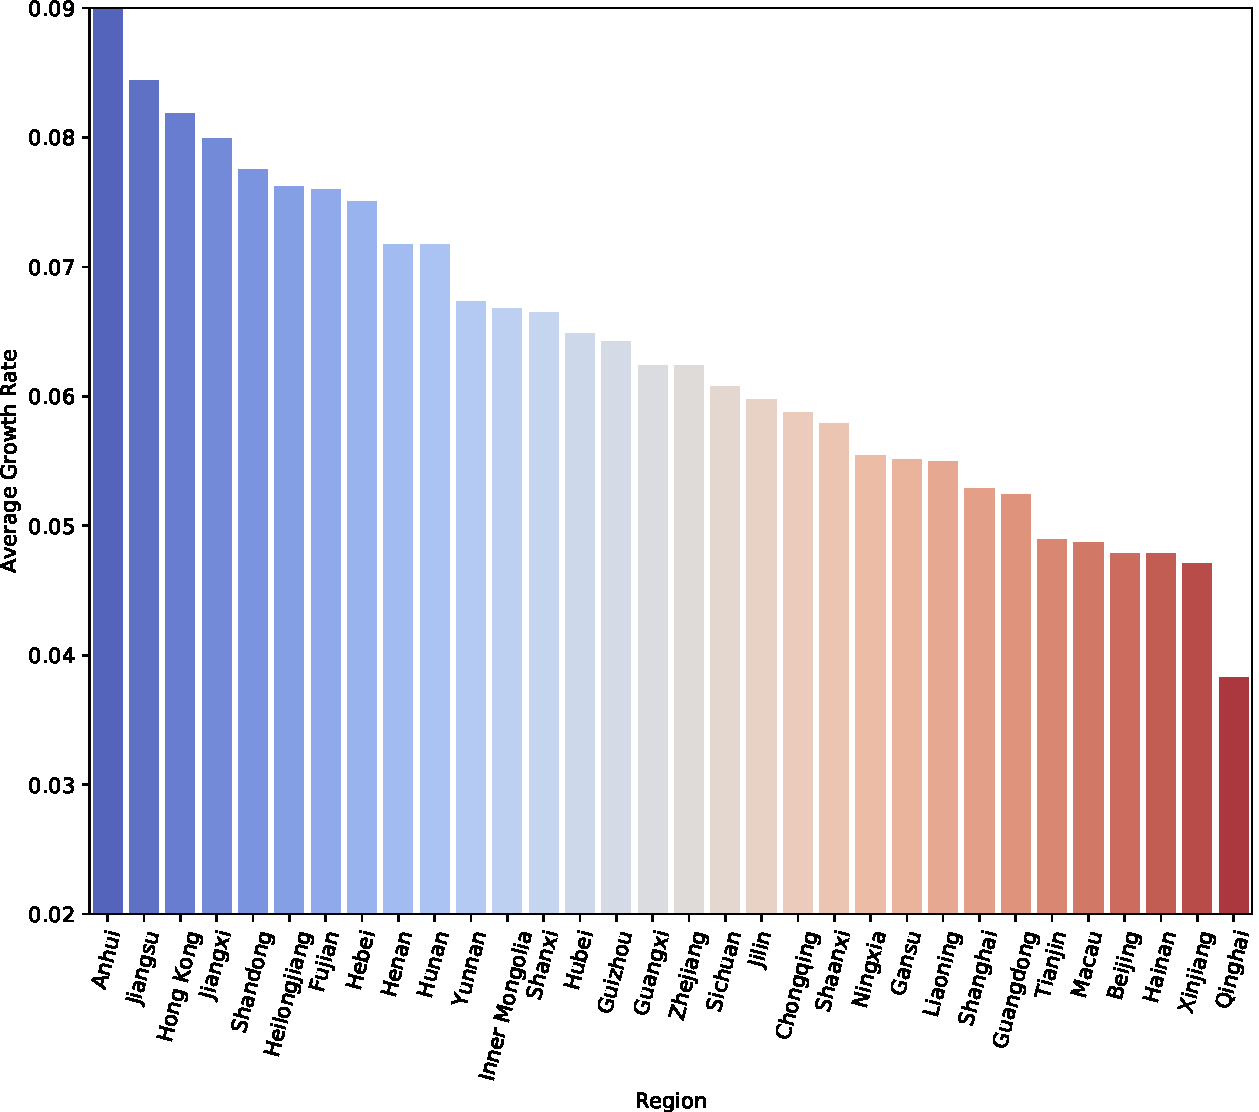
\includegraphics[width=0.8\textwidth]{ly1.pdf}
  \caption{Average Growth Rate of COVID-19 in China}
  \label{fig:ly1}
\end{figure}

Next, we examined the correlation between the average growth rate and the geographical distance to Hubei, the outbreak city of COVID-19. Our conjecture is the average growth rate decreases with an increase in distance. The geographical distance is calculated via the Geopy python library~\cite{geopy}. \cref{fig:ly2} shows the average growth rate by distance to Hubei. The trend matches our expectations. For regions within 1000 km from Hubei, their average growth rate is greater than those distant regions. However, we still observed some counterexamples, for instance, Heilongjiang. Heilongjiang is China's northernmost province which shares a border with Russia, while Hubei is a landlocked province in central China. To figure out possible explanations for Heilongjiang's high average growth rate, we did a literature research for COVID-19 news in Heilongjiang. We found that since early April, there were a large number of imported COID-19 cases from Russia~\cite{heilongjiang}. It is highly possible that these imported cases result in an increase of COVID-19's growth rate.
\begin{figure}[htp]
  \centering
  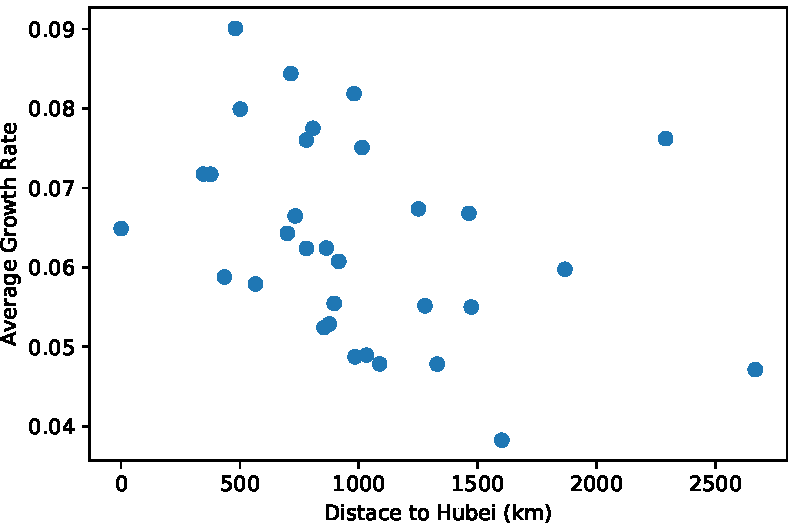
\includegraphics[width=0.6\textwidth]{ly2.pdf}
  \caption{Average Growth Rate by Distance to Hubei}
  \label{fig:ly2}
\end{figure}

Apart from~\cref{fig:ly2}, we also calculated the covariance matrix for the average growth rate and distance (we cannot apply ANOVA here since the average growth rate is not normally distributed). The result is shown in~\cref{eq:3}, where the negative covariance indicates a negative correlation between the two variables.
\begin{equation}
    \bm{cov}(\bm{AverageGrowthRate}, \bm{Distance}) = 
    \begin{bmatrix}
        1.58403777e-04 & -2.48454066e+00 \\
        -2.48454066e+00 & 3.08315655e+05
    \end{bmatrix}\label{eq:3}
\end{equation}

The last analysis we conducted on the COVID-19 Open Research dataset is the ANOVA between the daily growth rates and weather data. We chose four regions for this analysis: Beijing, Guangdong, Liaoning, and Shanghai. These four provinces are located in different areas in China, so that their weather data is distinct. The corresponding mean of the daily growth rate is labeled as $\mu_1$, $\mu_2$, $\mu_3$, and $\mu_4$. For each pair of weather data, a two-way ANOVA is carried out to verify the following hypothesis test:
    \begin{align}
        H_0: & \:\mu_1 = \mu2 = \mu3 = \mu4 \\
        H_1: & \:\mathit{at\:least\:one\:mean\:differs\:from\:others}
    \end{align}

In~\cref{tab:ly3}, we display the result of ANOVA for the mean temperature and total precipitation. It demonstrates that there is no significant difference between growth with distinct mean temperature and total precipitation. For other weather data, the results are similar. Since~\cref{fig:ly2} also illustrates that the average growth rate is between 0.04 - 0.09, which is quite a small range, we can conclude that the weather data has little effect on the spread of COVID-19.

% Please add the following required packages to your document preamble:
% \usepackage{graphicx}
\begin{table}[]
\centering
\caption{ANOVA Result for Mean Temperature and Total Precipitation}
\label{tab:ly3}
\resizebox{0.6\textwidth}{!}{%
\begin{tabular}{lrrrr}
\hline
\multicolumn{1}{c}{\textbf{Measure}} & \multicolumn{1}{c}{\textbf{sum\_sq}} & \multicolumn{1}{c}{\textbf{df}} & \multicolumn{1}{c}{\textbf{F}} & \multicolumn{1}{c}{\textbf{PR(\textgreater{}F)}} \\
\hline
C(temp) & 8.453343e-17 & 2.0 & 7.406908e-16 & 1.000000 \\
C(prcp) & 3.274350e-18 & 2.0 & 2.869020e-17 & 1.000000 \\
C(temp):C(prcp) & 4.702349e-02 & 4.0 & 2.060124e-01 & 0.813969 \\
Residual & 1.352415e+01 & 237.0 & NaN & NaN \\
\hline
\end{tabular}%
}
\end{table}
